\section{Введение в теорию евклидовых пространств.}
\begin{definition}
    Пусть $E = (E, \langle \cdot, \cdot \rangle)$~---~евклидово пространство. Пусть $\{e_n\}_{n = 1}^{+\infty}$~---~ортогональная система из ненулевых векторов в нём.
    Тогда $\forall f \in E$ будем называть
    \begin{equation*}
        \alpha_k(f) = \dfrac{\langle f, e_k \rangle}{\langle e_k, e_k \rangle}, k \in \N.
    \end{equation*}
    коэффициентом Фурье элемента $f$ по системе $\{e_n\}_{n = 1}^{+\infty}$.
\end{definition}
\begin{theorem}[минимальное свойство коэффициентов Фурье]
    Пусть $E = (E, \langle \cdot, \cdot \rangle)$~---~евклидово пространство. Тогда $\forall f \in E \hookrightarrow$
    \begin{equation*}
        \inf\limits_{\beta_1, \ldots, \beta_n} \bigr\|f - \sum\limits_{k = 1}^n \beta_k e_k\bigr\| = \bigr\|f - \sum\limits_{k = 1}^n \alpha_k(f)e_k\bigr\|.
    \end{equation*}
\end{theorem}
\begin{proof}
    Пусть $d_n = \sum\limits_{k = 1}^n (\alpha_k(f) - \beta_k) e_k$, где $\beta_i$~---~произвольные вещественные коэффициенты.
    Тогда
    \begin{multline*}
        \big\|f - \sum\limits_{k = 1}^n \beta_{k}e_k\big\|^2 = \big\|f - S_n[f] + S_n[f] - \sum\limits_{k = 1}^n \beta_k e_k\big\|^2 = \\ =
        \langle f - S_n + d_n, f - S_n + d_n \rangle = \langle f - S_n, f - S_n \rangle + 2 \langle d_n, f - S_n \rangle + \langle d_n, d_n \rangle,
    \end{multline*}
    Где под $S_n[f]$ понимается $n$-ая сумма ряда Фурье, то есть $S_n[f] = \sum\limits_{k = 1}^n a_k(f)e_k$.
    Заметим, что $\forall k \in \{1, \ldots, n\}$ верно, что
    \[
        \langle e_k, f - S_n[f] \rangle = \langle e_k, f \rangle - \langle e_k, S_n[f] \rangle = \langle e_k, f \rangle - \langle e_k, \alpha_k(f)e_k \rangle = 0.
    \]
    Значит $2\langle d_n, f - S_n \rangle = 0$, и квадрат отклонения выражается как
    \begin{equation*}
        \big\|f - \sum\limits_{k = 1}^n \beta_k e_k\big\|^2 = \langle f - S_n, f - S_n \rangle+ \langle d_n, d_n \rangle \geq \langle f, f \rangle,
    \end{equation*}
    причём минимум достигается при $d_n = 0$.
    Но, тогда, из ортогональности системы и определения $d_n$, мы получаем что $\forall n \in \N$
    \begin{equation*}
        \big\|f - S_n[f]\big\| \leq \big\|f - \sum\limits_{k = 1}^n \beta_k e_k\big\|.
    \end{equation*}
    для всяких $\{\beta_i\}$. То есть
    \[
        \big\|f - S_n[f]\big\| \leq \inf\limits_{\beta_i \in \R, i = \overline{1, k}} \big\|f - \sum\limits_{k = 1}^n \beta_{k}e_k\big\|.
    \]
    Поскольку $S_n[f] = \sum\limits_{k = 1}^n a_k(f)e_k$, то утверждение теоремы доказано.
\end{proof}
\begin{note}[Геометрическая интерпретация теоремы]
    Мы рассматриваем линейную оболочку базисных векторов $\text{Lin}\{e_1,\dots,e_n\}$. Рассматрива произвольный вектор $f$, то среди всех возможных комбинаций наилучшее приближение дает именно сумма Фурье. Те $S_n[f]$ это просто ортогональная проекция $f$ на линейную оболочку. Это является ортогональной проекцией в силу того, что $ \langle e_k, f - S_n[f] \rangle = 0.$

    \begin{minipage}{\textwidth}
    \centering
    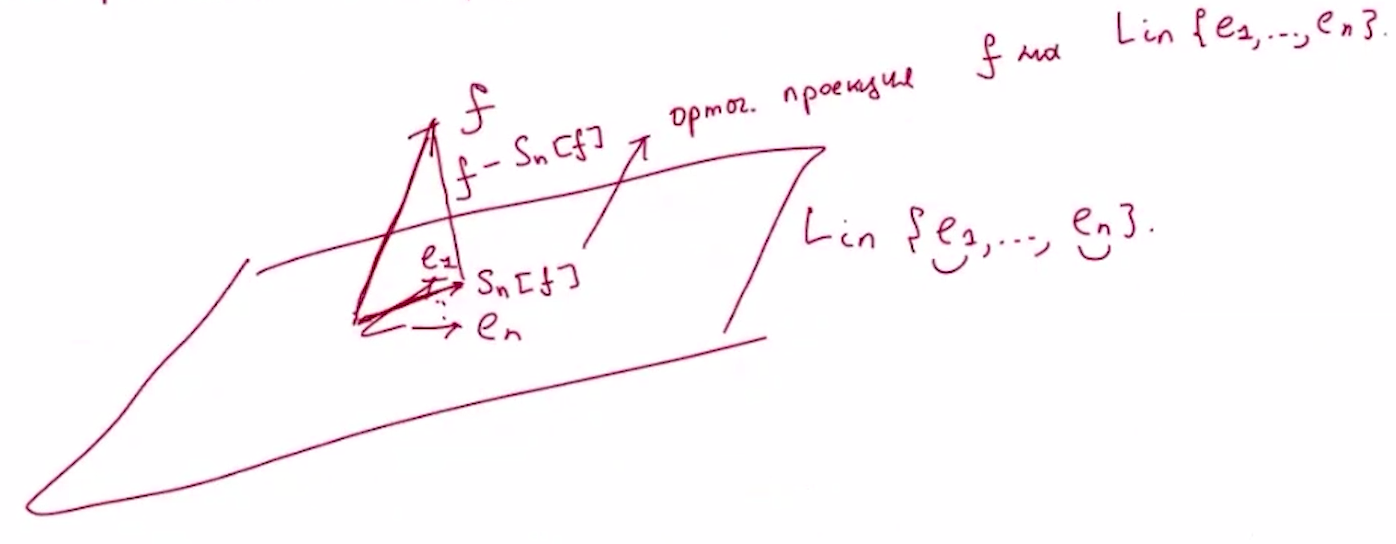
\includegraphics[width=0.7\textwidth]{Pictures/pic1.png} 
    \end{minipage}



\end{note}
\begin{theorem}[О единственности]
    Пусть $E = (E, \langle \cdot, \cdot \rangle)$~---~евклидово пространство и $f \in E$.
    Пусть $\{e_n\}_{n = 1}^{+\infty}$~---~ортогональная система в $E$ и $f = \sum\limits_{k = 1}^{+\infty} \alpha_k e_k$ (где сходимость ряда понимается в смысле нормы)
    Тогда $\forall k \in \N \alpha_k$~---~коэффициент Фурье $f$.
\end{theorem}
\begin{proof}
    Пусть $S_n = \sum\limits_{k = 1}^n \alpha_k e_k$.
    Тогда
    \[
        |\langle f, e_k \rangle - \langle S_n, e_k \rangle| = |\langle f - S_n, e_k \rangle| \leq \|f - S_n\|\|e_k\| \rightarrow 0, n \rightarrow +\infty.
    \]
    А значит $\forall k \in \N \ \exists \lim\limits_{n \ra +\infty} \langle S_n, e_k \rangle = \langle f, e_k \rangle$.
    В силу ортогональности системы мы получаем искомое утверждение.
\end{proof}
\begin{lemma}
    Пусть дано $E = (E, \langle \cdot, \cdot \rangle)$~---~евклидово пространство и $\{e_n\}_{n = 1}^{+\infty}$~---~ортогональная система в нём.
    Тогда $\forall n \in \N$ справедливо следующее:
    \[
        \|f\|^2 = \|f - S_n[f]\|^2 + \sum\limits_{k = 1}^n \alpha_k^2(f)\langle e_k, e_k \rangle
    \]
\end{lemma}
\begin{proof}
    Доказательство очевидно в силу ортогональности системы и линейности скалярного произведения.
\end{proof}
\begin{corollary}[Неравенство Бесселя]
    В условиях предыдущей леммы $\forall f \in E$ справедливо неравенство Бесселя
\[
\sum_{k=1}^\infty \bigl|\langle f,\,e_k\rangle\bigr|^2 \;\le\;\|f\|^2.
\]

\end{corollary}
\begin{proof}
    В силу предыдущей леммы и неотрицательности нормы $\forall n \in \N \hookrightarrow$
    \[
        \sum\limits_{k = 1}^n \alpha_k^2(f)\|e_k\|^2 \leq \|f\|^2.
    \]
    Взятие супремума по $n \in \N$ завершает доказательство.
\end{proof}
\begin{theorem}[Рисс, Фишер]
    Пусть $H = (H, \langle \cdot, \cdot \rangle)$~---~гильбертово пространство (то есть полное относительно нормы евклидово пространство).
    Пусть $\{e_n\}_{n = 1}^{+\infty}$~---~ортогональная система в нём.
    Тогда следующие условия эквивалентны:
    \begin{enumerate}
        \item $\sum\limits_{k = 1}^{+\infty} \alpha_k e_k$ сходится к некоторому элементу $f \in H$ в смысле евклидовой нормы.
        \item Для некоторой $f \in H$ выполняется $\alpha_k = \alpha_k(f)$ при всяком натуральном $k$.
        \item Числовой ряд $\sum\limits_{k = 1}^{+\infty} |\alpha_k|^2\|e_k\|^2$~---~сходится.
    \end{enumerate}
\end{theorem}
\begin{proof}
    Импликация $1) \Rightarrow 2)$ очевидна в силу теоремы о единственности: $\alpha_k$ будут просто коэффициентами Фурье своей суммы. \\
    Импликация $2) \Rightarrow 3)$ очевидна в силу неравенства Бесселя. \\
    Покажем что $3) \Rightarrow 1)$.
    Пусть, без ограничения общности, $m$ и $n$~---~натуральные и $m > n$.
    Тогда
    \begin{equation*}
        \bigr\langle \sum\limits_{k = n}^{m} \alpha_k e_k, \sum\limits_{k = n}^m \alpha_k e_k \bigr\rangle = \big\|\sum\limits_{k = n}^m \alpha_k e_k\big\|.
    \end{equation*}
    В силу ортогональности системы и Критерия Коши сходимости числового ряда
    \[
        \sum\limits_{k = n}^m |\alpha_k|^2\|e_k\|^2 \rightarrow 0, n, m \ra +\infty.
    \]
    Тогда последовательность частичных сумм ряда фундаментальна и он сходится к $f \in H$, поскольку $H$~---~полно.
    Импликация доказана.
\end{proof}
\begin{definition}
    Пусть $E = (E,  \|\cdot\|)$~---~ЛНП.
    Система векторов $\{e_n\}_{n = 1}^{+\infty}$ называется полной в $E$, если $\forall f \ \forall \epsilon > 0 \exists c_1, \ldots, c_n \in \R$
    такая, что $\|f - \sum\limits_{k = 1}^n c_k e_k\| < \epsilon$.
\end{definition}
\begin{note}
    Всякий базис Шаудера является полной системой.
    Обратное неверно: контрпримером является $\{x^n\}_{n = 0}^{+\infty}$ в $C([-1, 1])$.
    Она полна по теореме Вейерштрасса, но не является базисом.
    Предположим противное.
    Тогда для
    \[
        f(x) = |x| \exists ! \{c_k\}_{k = 0}^{+\infty}: |x| = \sum\limits_{k = 0}^{+\infty} c_k x^k.
    \]
    причём равенство понимается в равномерном смысле.
    Но тогда по теореме о дифференцируемости степенного ряда мы получаем дифференцируемость $f$ в нуле -- противоречие.
\end{note}
\begin{definition}
    Пусть $E = (E, \langle \cdot, \cdot \rangle)$~---~евклидово пространство.
    Ортоональная система $\{e_n\}_{n = 1}^{+\infty}$ называется замкнутой, если из ортогональности $f$ каждому $e_k$ следует то, что $f = 0$.
\end{definition}
\begin{theorem}[<<Основная>> теорема.]
    Пусть $H = (H, \langle \cdot, \cdot \rangle)$~---~гильбертово пространство.
    Пусть $\{e_k\}_{k = 0}^{+\infty}$~---~ортогональная система в нём.
    Следующие условия эквивалентны:
    \begin{enumerate}
        \item Система $\{e_n\}_{n = 1}^{+\infty}$~---~полна.
        \item Система $\{e_n\}_{n = 1}^{+\infty}$~---~базис.
        \item $\forall f \in H$ ряд Фурье по системе $\{e_k\}$ сходится к $f$.
        \item Справедливо равенство Парсеваля:
        \[
            \|f\|^2 = \sum\limits_{k = 1}^{+\infty} |\alpha_k|^2 \|e_k\|^2.
        \]
        \item Система $\{e_n\}_{n = 1}^{+\infty}$~---~замкнута.
    \end{enumerate}
\end{theorem}
\begin{proof}
    Покажем импликацию $1) \Rightarrow 2)$. \\
    Пусть $\Delta_n = \inf\limits_{\beta_1, \ldots, \beta_n} \big\|f - \sum\limits_{k = 1}^n \beta_k e_k \big\|, n \in \N$.
    Нетрудно заметить, что $\Delta_{n + 1} \leq \Delta_n \forall n \in \N$, поскольку занулением лишнего коэффициента сводится к предыдущей дельте.
    Тогда, из монотонности последовательности и неотрицательности каждого из её членов следует существование предела, равного инфинуму:
    \[
        \exists \lim\limits_{n \ra +\infty} \Delta_n = \inf\limits_n \Delta_n.
    \]
    Поскольку по определению полноты $\forall f \in H \forall \epsilon > 0 \exists n \in \N \exists c_1, \ldots, c_n \in \R:$
    \[
        \|f - \sum\limits_{k = 1}^n c_k e_k\| < \epsilon.
    \]
    то $\inf\limits_n \Delta_n = 0$.
    В силу минимального свойства коэффициентов Фурье $\Delta_n = \|f - S_n[f]\|$.
    А значит $\{e_n\}_{n = 1}^{+\infty}$~---~базис (из существования предела $\Delta_n$ и теоремы о единственности). \\
    Импликация $2) \Ra 3)$ верна по теореме о единственности -- эти коэффициенты в единственном разложении по базису и будут коэффициентами ряда Фурье. \\
    Импликация $3) \Ra 4)$ следует из ранее доказанной леммы:
    \[
        \|f\|^2 = \|f - S_n[f]\|^2 + \sum\limits_{k = 1}^n |\alpha_k(f) e_k|\langle e_k, e_k \rangle.
    \]
    При устремлении $n$ в бесконечность получаем равенство Парсеваля. \\
    Заметим, что та же самая лемма даёт нам из выполнения равенства Парсеваля базисность системы, а значит $4) \Ra 2$.
    Ранее было замечено, что из базисности системы векторов следует её полнота, то есть $2) \Ra 1)$.
    При этом, в вышеприведённых рассуждениях полнота нигде не использовалась, а значит $1), 2), 3), 4)$ эквивалентны и при условии отсутствия полноты. \\
    Покажем $4) \Ra 5)$.
    Пусть существует $f \in H$ такой, что $\forall k \in \N \hookrightarrow f \perp e_k$.
    Тогда $\forall k \in \N \alpha_k(f) = 0$ и $\|f\|^2 = 0$ по равенству Парсеваля.
    По определению нормы $f = 0$ и система замкнута. \\
    Покажем $5) \Ra 1)$.
    Зафиксируем $f \in H$.
    Из неравенства Бесселя следует:
    \[
        \sum\limits_{k = 1}^{+\infty} |\alpha_k(f)|\|e_k\|^2 \leq \|f\|^2 < +\infty.
    \]
    По теореме Рисса-Фишера ряд $\sum\limits_{k = 1}^{+\infty} \alpha_k(f) e_k$ сходится к некоторому элементу $S \in H$.
    Заметим, что $\langle S, e_k \rangle = \alpha_k(f) \langle e_k, e_k \rangle$~---~по теореме о единственности.
    Тогда $\langle S, e_k \rangle = \langle f, e_k \rangle \forall k \in \N$.
    Из замкнутости системы $\{e_k\}$ следует что $S - f = 0 \Ra S = f$ и теорема доказана.
\end{proof}
\begin{note}
    В неполных евклидовых пространствах система может быть замкнута, но не полна. \\
    Введём обозначение $e_k = (0, \ldots, 1, 0, \ldots,)$ (где $1$ стоит на $k$-ом месте). \\
    И пусть $e = (1, 1/2, 1/3, \ldots, 1/n, \ldots)$.
    Рассмотрим тогда подпространство $l_2$, которое обозначим за $E$ и определим как
    \[
        E = Lin(e, e_2, e_3, \ldots).
    \]
    с индуцированным скалярным произведением.
    Очевидно, что $E$~---~неполно:
    \[
        \|\left(e - \sum\limits_{k = 2}^n \dfrac{e_k}{k}\right) - e_1\| \ra 0, n \ra +\infty.
    \]
    но $e_1 \notin E$. \\
    В $E$ система $\{e_2, e_3, \ldots\}$~---~замкнута (вектор $(c, 0, \ldots) \notin E$, а значит если вектор ортогонален всем $e_k$, то он равен 0), но не полна ($e$ не выражается через $e_k$).
\end{note}

% Возможно, я тут при техе что-то забыл; речекнуть лекцию.
